%
% m-1dim.tex -- ein eindimensionales Beispiel
%
% (c) 2017 Prof Dr Andreas Müller, Hochschule Rapperswil
%
\section{Ein eindimensionales Beispiel%
\label{skript:multipol:1dimbeispiel}}
\rhead{Ein eindimensionales Beispiel}
In diesem Abschnitt betrachten wir eine Funktion, die nur von einer
Variablen $x$ abhängt.
Ausserdem interessiert uns in erster Linie das Verhalten der Funktion
für $x\to\pm\infty$.
Wir verwenden dazu eine Methode, die sich leicht auf die dreidimensionale
Situation ausweiten lässt.

\subsection{Monopol und Dipol}
Das Potential einer Ladung $e$ fällt mit der Entfernung $r$ nach dem
Coulomb-Gesetz
\index{Coulomb-Gesetz}%
\[
f(r)=\frac1{4\pi\varepsilon_0}\frac{q}r
\]
ab.
Platziert man die Ladung $q$ im Punkt $a$ eines eindimensionalen
Koordinatensystems, dann ist das Potential in Abhängigkeit von $x$
\begin{equation}
f_1(x) = \frac{q}{4\pi\varepsilon_0} \frac1{|x-a|}.
\label{skript:multipol:1monopol}
\end{equation}
Für $x>a$ kann man \eqref{skript:multipol:1monopol} schreiben als
\begin{equation}
f_1(x)
=
\frac{q}{4\pi\varepsilon_0} \frac1{x-a}
=
\frac{q}{4\pi\varepsilon_0} \frac1x\frac1{1-\displaystyle\frac{a\mathstrut}{x}}.
\label{skript:multipol:1abfall}
\end{equation}
Im letzten Faktor kann man ablesen, dass der Summand $a/x$ im Nenner
auf der rechten Seite für grosse $x$ unbedeutend wird, so dass $f(x)$
immer noch wie $1/x$ abfällt, unabhängig davon, wo die Ladung platziert
wird.

\begin{figure}
\centering
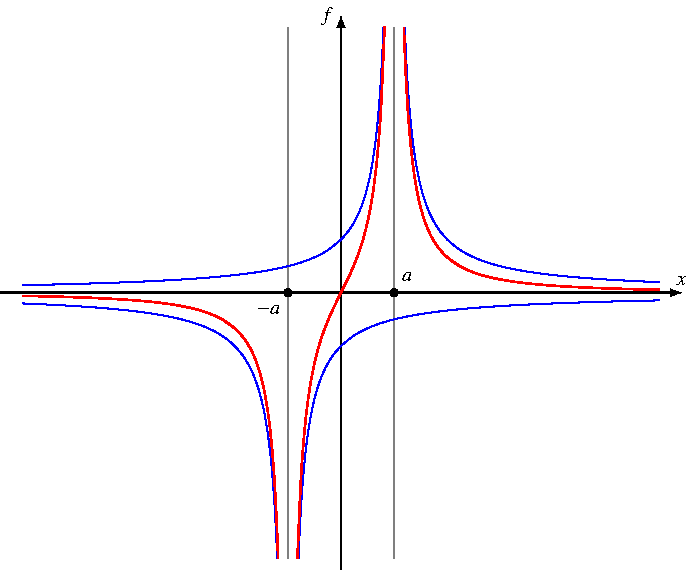
\includegraphics{chapters/tikz/dipol1.pdf}
\caption{Potential
\eqref{skript:multipol:1dipol}
des eindimensionalen Dipols
\label{skript:multipol:figure:1dim}}
\end{figure}

Zwei entgegengesetzte Punktladungen an den Stellen $x=\pm a$ haben also
das Potential
\begin{equation}
f_2(x)
=
\frac1{4\pi\varepsilon_0}\frac{q}{|x+a|}
-
\frac1{4\pi\varepsilon_0}\frac{q}{|x-a|}
=
\frac{q}{4\pi\varepsilon_0}\biggl( \frac1{|x+a|} - \frac1{|x-a|} \biggr).
\label{skript:multipol:1dipol}
\end{equation}
(Abbildung~\ref{skript:multipol:figure:1dim}).
Wir sind nur an den Funktionswerten interessiert für $x$-Werte, die
wesentlich grösser sind als $a$, als in grosser Entfernung von
den Ladungen.
Wir interessieren uns also für $x$-Werte so, dass $x/a$ sehr gross ist,
oder umgekehrt dass $a/x$ sehr klein ist.

Wenn man in Gleichung \eqref{skript:multipol:1dipol} das Vorzeichen
von $x$ kehrt, dann ändert das Vorzeichen von $f$, also $f_2(-x)=-f_2(x)$,
$f$ ist eine ungerade Funktion.
Es reicht daher, die Funktion $f_2(x)$ für $x\gg a$ zu untersuchen.

Verwenden wir die Gleichung \eqref{skript:multipol:1abfall} in $f_2(x)$,
erhalten wir
\begin{align}
f_2(x)
&=
\frac{q}{4\pi\varepsilon_0}\biggl(\frac1{x+a}-\frac1{x-a}\biggr)
=
\frac{q}{4\pi\varepsilon_0}\cdot\frac1x\cdot\biggl(
\frac1{1+\frac{a\mathstrut}{x}}
-
\frac1{1-\frac{a\mathstrut}{x}}
\biggr)
=
\frac{q}{4\pi\varepsilon_0}\cdot\frac1x\cdot
\frac{\bigl(1-\frac{a}{x}\bigr)-\bigl(1+\frac{a}{x}\bigr)}{1-\frac{a^2}{x^2}}
\notag
\\
&=
\frac{q}{4\pi\varepsilon_0}\cdot\frac1x\cdot
\biggl(-\frac{2a}{x}\biggr)
\cdot
\frac1{1-\frac{a^2}{x^2}}
=
-\frac{qa}{2\pi\varepsilon_0}\cdot\frac1{x^2}\cdot\frac{1}{1-\frac{a^2}{x^2}}.
\label{skript:multipol:2abfall}
\end{align}
Der Term $a^2/x^2$ im Nenner des letzten Faktors ist für grosse Werte von
$x$ wieder unbedeutend.
Der dominierende Term für das Verhalten für grosse $x$ ist daher der
Faktor $1/x^2$.

Ein weiterer interessanter Aspekt der Formel~\eqref{skript:multipol:2abfall}
ist, dass nur noch die Kombination $qa$ von Ladung und Abstand der Ladungen
vorkommt.
Das Fernfeld für grosse Werte von $x$ ändert also nicht, wenn wir $a$
kleiner machen, aber gleichzeitig $q$ vergrössern, so dass das Produkt
$qa$ konstant bleibt.
Man nennt $d=2qa$ das {\em Dipolmoment} der beiden Ladungen.
\index{Dipolmoment}%
Der Dipol mit Dipolmoment $d$ hat daher für grosse $x$ das Potential
\[
f_2(x)
=
-\frac{d}{4\pi\varepsilon_0}\cdot \frac1{x^2}\cdot \frac1{1-\frac{a^2}{x^2}}
\simeq
-\frac{d}{4\pi\varepsilon_0}\cdot \frac1{x^2}.
\]

Aus diesen Beispielen können wir die Vermutung ableiten, dass weitere
Terme die Form
\[
-\frac{b}{4\pi\varepsilon_0}\cdot\frac1{x^k}
\]
haben müssen, wobei $b$ die Dimension einer Ladung mal die $(k-1)$-te
Potenz einer Distanz sein muss.

\subsection{Stetige Ladungsverteilung%
\label{skript:multipol:section:stetigeladungsverteilung}}
Betrachten wir jetzt statt zweier Ladungen eine beliebige 
Ladungsverteilung $\varrho(x)$, die aber ausserhalb des Intervalls
$[-a,a]$ verschwindet, also $\varrho(x)=0$ für $|x|>a$.
Stellen wir uns die Ladungsverteilung als eine Überlagerung einzelner
Ladungen an Positionen $y\in[-a,a]$ vor, dann k"onnen wir das
Potential des Fernfeldes sofort aus~\eqref{skript:multipol:2abfall}
ableiten:
\[
f(x)
\simeq
\frac{1}{4\pi\varepsilon_0}
\underbrace{\int_{-a}^a \varrho(y)\,dy }_{\displaystyle =q}
\frac1x
+
\frac{1}{4\pi\varepsilon_0}
\underbrace{\int_{-a}^a \varrho(y)y \,dy}_{\displaystyle =d}
\frac1{x^2}
+
\dots
=
\frac{1}{4\pi\varepsilon_0}
\sum_{k=0}^\infty
\frac1{x^{k+1}} 
\int_{-a}^a\varrho(y)y^k\,dy
\]
Der erste Term ist das Potential einer Punktladung $q$ im Ursprung, der
zweite das Dipolpotential eines Dipols mit Dipolmoment $d$.
Wir nennen den ersten Term auch den {\em Monopolterm}.
\index{Monopol}%

Die Integrale 
\[
b_k=\int_{-a}^a \varrho(y)\,y^k\,dy
\]
heissen die {\em $k$-ten Momente} der Verteilung $\varrho$.
\index{Moment einer Funktion}%
Die $k$-ten Momente bestimmen also die Darstellung des Fernfeldes
einer Ladungsverteilung vollständig durch die Formel
\[
f(x)
\simeq
\frac1{4\pi\varepsilon_0}\sum_{k=0}^\infty b_k\frac{1}{x^{k+1}}.
\]
Wir behaupten nicht, dass die Summe auf der rechten Seite mit dem Potential
der Ladungsverteilung übereinstimmen.
Vielmehr ist die Summe eine Zerlegung des Feldes
nach ``Abfalls-Geschwindigkeit'' in grosser Entfernung,
ganz ähnlich wie die Fourier-Koeffizienten einer im Intervall
$[-\pi,\pi]$ definierten Funktion $f(x)$
\[
a_k=\frac1{2\pi}\int_{-\pi}^\pi f(x)\cos kx\,dx
\qquad\text{und}\qquad
b_k=\frac1{2\pi}\int_{-\pi}^\pi f(x)\sin kx\,dx
\]
eine Analyse nach Frequenzen bilden.
Die Fourierreihe
\[
\frac{a_0}2+\sum_{k=1}^\infty (a_k\cos kx+b_k\sin kx)
\]
ist eine periodische Funktion auf der ganzen reellen Achse, die
im Intervall $[-\pi,\pi]$ mit der ursprünglichen Funktion übereinstimmt.
Die Summe stimmt also mit der ursprünglichen Funktion nicht direkt
überein.

\subsection{Geometrische Reihe%
\label{skript:multipol:section:geometrischereihe}}
Bei der Analyse sowohl einer um $a$ verschobenen Einzelladung sowie auch
des Dipols aus zwei Ladungen bei $\pm a$ haben wir am Schluss Terme der
Form
\[
\frac1{1-\displaystyle\frac{a}{x}}
\qquad\text{bzw.}\qquad
\frac1{1-\displaystyle\frac{a^2}{x^2}}
\]
vernachlässigt.
Wir suchen nach einer Möglichkeit, diese Terme exakt zu berücksichtigen,
und trotzdem nur eine einfache Potenzreihe zu bekommen.

In der Analysis lernt man, die Summe der {\em geometrische Reihe}
\index{geometrische Reihe}
\index{Reihe, geometrische}
\[
s=a+aq+aq^2+\dots + aq^n
\]
zu berechnen.
Dazu bildet man $qs - s$ und findet
\begin{align*}
qs-s
=
s(q-1)
&=
q(a+aq+aq^2+\dots + aq^n)-(a+aq+aq^2+\dots + aq^n)
\\
&=
a(q+q^2+q^3\dots+q^{n+1}-1-q-q^2-\dots-q^n)
=
a(q^{n+1}-1)
\end{align*}
und schliesst
\[
s=a\frac{q^{n+1}-1}{q-1}.
\]
Wenn $|q|<1$ ist, dann kann man die Summe für beliebig grosse $n$ bilden,
und bekommt im Grenzwert $n\to\infty$
\begin{equation}
\sum_{k=0}^\infty aq^k = a\frac{1}{1-q}.
\label{skript:multipol:geom}
\end{equation}
Wir können diese Formel verwenden, um die bisher vernachlässigten Terme
exakt wiederzugeben:
\begin{align*}
\frac{1}{1-\displaystyle\frac{a}{x}}
&=
1+\frac{a}{x}+\frac{a^2}{x^2}+\dots
=
\sum_{k=0}^\infty \frac{a^k}{x^k}
\\
\frac{1}{1-\displaystyle\frac{a^2}{x^2}}
&=
1+\frac{a^2}{x^2}+\frac{a^4}{x^4}+\dots
=
\sum_{k=0}^\infty \frac{a^{2k}}{x^{2k}}
\\
\frac{1}{1+\displaystyle\frac{a^2}{x^2}}
&=
1-\frac{a^2}{x^2}+\frac{a^4}{x^4}-\dots
=
\sum_{k=0}^\infty (-1)^k\frac{a^{2k}}{x^{2k}}.
\end{align*}
Die letzte Formel erhält man, indem man in \eqref{skript:multipol:geom}
$q$ durch $-q$ ersetzt und dann $q=a^2/x^2$ einsetzt.

Wir wenden dies jetzt wieder auf eine Ladungsverteilung
$\varrho(y)$ im Intervall $[-a,a]$ an.
Das Potential einer Einheitsladung an der Stelle $y$ ist
\[
f_y(x)
=
\frac1{4\pi\varepsilon_0}\cdot \frac{1}{x}\cdot\frac{1}{1-\displaystyle\frac{x}{y}}
=
\frac1{4\pi\varepsilon_0}\cdot \frac{1}{x}
\sum_{k=0}^\infty \frac{y^k}{x^k}
=
\frac1{4\pi\varepsilon_0}
\sum_{k=0}^\infty \frac{y^k}{x^{k+1}}.
\]
Durch Überlagerung mit Hilfe der Ladungsverteilung $\varrho(y)$ 
erhalten wir die exakte Formel für das Potential der Ladungsverteilung
\begin{equation}
f(x)
=
\int_{-a}^af_y(x)\,dy
=
\frac{1}{4\pi\varepsilon_0}
\sum_{k=0}^\infty
\frac{1}{x^{k+1}}
\underbrace{\int_{-a}^a\varrho(y)\,y^k\,dy}_{\displaystyle =b_k}
\cdot
=
\frac{1}{4\pi\varepsilon_0}
\sum_{k=0}^\infty b_k
\frac{1}{x^{k+1}},
\label{skript:multipol:reiheexakte}
\end{equation}
wobei die $b_k$ wieder die $k$-ten Momente der Ladungsverteilung
$\varrho(y)$ sind.

Es stellt sich also heraus, dass die in
Abschnitt~\ref{skript:multipol:section:stetigeladungsverteilung}
erratene Entwicklung sogar eine exakte Darstellung ist.
Bricht man die Reihe~\eqref{skript:multipol:reiheexakte} nach zwei
Termen ab, erhält man die Monopol- und Dipol-Komponenten des
Fernfeldes.
Alle späteren Terme der Reihe beschreiben die feineren Strukturen
der Ladungsverteilung und fallen so rasch mit der Entfernung ab,
dass sie für grosse Entfernungen vernachlässigt werde können.

Bei der Diskussion des Dipolmoments haben wir festgestellt, dass das
Fernfeld nur von der Grösse $d=2aq$ abhängt.
Verkleinert man den Abstand $a$ und vergrössert man gleichzeitig $q$,
so dass $d$ gleich gross bleibt, dann ändert sich das Fernfeld nicht.
Die Reihe~\eqref{skript:multipol:reiheexakte} verallgemeinert diese
Aussage auf eine beliebige Ladungsverteilung.
Ändern wir die Ladungsverteilung, achten aber darauf, dass die
$k$-ten Momente gleich bleiben, dann ändert sich das ausserhalb der
Ladungsverteilung messbare Potential nicht.
Die $k$-ten Momente beschreiben das ausserhalb der Ladungsverteilung
messbare Potential vollständig.

\subsection{Taylor-Reihe und Laurent-Reihe}
Im vorangegangenen Abschnitt haben wir gesehen, dass für grosse Werte von
$x$ die zur Diskussion stehende Funktion im Wesentlichen als Reihe
der inverse Potenzen $1/x^k$ beschrieben werden kann, also
\[
f(x)=\sum_{k=0}^\infty b_k\frac1{x^{k+1}}
\]
werden.
Schreiben wir $z=1/x$, dann wird daraus eine gewöhnliche Potenzreihe
\[
\tilde f(z)=\sum_{k=0}^\infty b_k z^{k+1}.
\]
Wenn die Funktion $z\mapsto \tilde f(z)$ differenzierbar ist, dann
können die Koeffizienten $b_k$ aus den Ableitungen der Funktion
$\tilde f$ gefunden
\begin{equation}
b_k=\frac{\tilde f^{(k)}(0)}{k!}
\qquad\Rightarrow\qquad
\tilde f(z)
=
\sum_{k=0}^\infty \frac{\tilde f^{(k)}(0)}{k!}z^k.
\end{equation}
Wir können dies betrachten als die Taylorreihe der Funktion $f$ um
den Punkt $\infty$.
\index{Taylor-Reihe}

Man nennt eine Reihe der Form
\[
\sum_{k=-\infty}^{\infty} (z-a)^k
\]
eine {\em Laurent-Reihe} im Punkt $a$.
\index{Laurent-Reihe}
Offensichtlich ist der Funktionswert in $z=a$ nicht definiert, und
oft wird die Reihe auch in einer Umgebung von $a$ nicht konvergieren.
Sie ist aber hervorragend dazu geeignet, das Verhalten einer Funktion
zu analysieren, die im Punkt $a$ eine Singularität aufweist.
Besonders nützlich ist sie dann, wenn $z$ komplex ist, denn man
kann zeigen, dass jede komplex differenzierbare Funktion mit einer
Singularität im Punkt $a$ in einer Umgebung von $a$ als Laurent-Reihe
dargestellt werden kann \cite{skript:mathsemdgl}.

Wenn wir also in der Lage sind, das eindimensionale Beispiel auf höhere
Dimensionen zu verallgemeinern, dann haben wir auch eine Verallgemeinerung
der Idee einer Taylorreihe um den Punkt $\infty$ auf höhere Dimensionen
gefunden.








